%\documentclass[times, 10pt,twocolumn]{article}
\documentclass[times,10pt,onecolumn]{article}
\usepackage{latex8}
\usepackage{times}
\usepackage{algorithm}
\usepackage{algorithmic}
\usepackage{amssymb}
\usepackage{psfrag,graphicx}
\usepackage{doublespace}
% Psfig/TeX 
\def\PsfigVersion{1.10}
\def\setDriver{\DvipsDriver} % \DvipsDriver or \OzTeXDriver
%
% All software, documentation, and related files in this distribution of
% psfig/tex are Copyright 1993 Trevor J. Darrell
%
% Permission is granted for use and non-profit distribution of psfig/tex 
% providing that this notice is clearly maintained. The right to
% distribute any portion of psfig/tex for profit or as part of any commercial
% product is specifically reserved for the author(s) of that portion.
%
% To use with LaTeX, use \documentstyle[psfig,...]{...}
% To use with TeX, use \input psfig.sty
%
% Bugs and improvements to trevor@media.mit.edu.
%
% Thanks to Ned Batchelder, Greg Hager (GDH), J. Daniel Smith (JDS),
% Tom Rokicki (TR), Robert Russell (RR), George V. Reilly (GVR),
% Ken McGlothlen (KHC), Baron Grey (BG), Gerhard Tobermann (GT).
% and all others who have contributed code and comments to this project!
%
% ======================================================================
% Modification History:
%
%  9 Oct 1990   JDS	used more robust bbox reading code from Tom Rokicki
% 29 Mar 1991   JDS	implemented rotation= option
% 25 Jun 1991   RR	if bb specified on cmd line don't check
%			for .ps file.
%  3 Jul 1991	JDS	check if file already read in once
%  4 Sep 1991	JDS	fixed incorrect computation of rotated
%			bounding box
% 25 Sep 1991	GVR	expanded synopsis of \psfig
% 14 Oct 1991	JDS	\fbox code from LaTeX so \psdraft works with TeX
%			changed \typeout to \ps@typeout
% 17 Oct 1991	JDS	added \psscalefirst and \psrotatefirst
% 23 Jun 1993   KHC     ``doclip'' must appear before ``rotate''
% 27 Oct 1993   TJD	removed printing of filename to avoid 
%			underscore problems. changed \frame to \fbox.
%			Added OzTeX support from BG. Added new
%			figure search path code from GT.
%
% ======================================================================
%
% Command synopsis:
%
% \psdraft	draws an outline box, but doesn't include the figure
%		in the DVI file.  Useful for previewing.
%
% \psfull	includes the figure in the DVI file (default).
%
% \psscalefirst width= or height= specifies the size of the figure
% 		before rotation.
% \psrotatefirst (default) width= or height= specifies the size of the
% 		 figure after rotation.  Asymetric figures will
% 		 appear to shrink.
%
% \psfigurepath{dir:dir:...}  sets the path to search for the figure
%
% \psfig
% usage: \psfig{file=, figure=, height=, width=,
%			bbllx=, bblly=, bburx=, bbury=,
%			rheight=, rwidth=, clip=, angle=, silent=}
%
%	"file" is the filename.  If no path name is specified and the
%		file is not found in the current directory,
%		it will be looked for in directory \psfigurepath.
%	"figure" is a synonym for "file".
%	By default, the width and height of the figure are taken from
%		the BoundingBox of the figure.
%	If "width" is specified, the figure is scaled so that it has
%		the specified width.  Its height changes proportionately.
%	If "height" is specified, the figure is scaled so that it has
%		the specified height.  Its width changes proportionately.
%	If both "width" and "height" are specified, the figure is scaled
%		anamorphically.
%	"bbllx", "bblly", "bburx", and "bbury" control the PostScript
%		BoundingBox.  If these four values are specified
%               *before* the "file" option, the PSFIG will not try to
%               open the PostScript file.
%	"rheight" and "rwidth" are the reserved height and width
%		of the figure, i.e., how big TeX actually thinks
%		the figure is.  They default to "width" and "height".
%	The "clip" option ensures that no portion of the figure will
%		appear outside its BoundingBox.  "clip=" is a switch and
%		takes no value, but the `=' must be present.
%	The "angle" option specifies the angle of rotation (degrees, ccw).
%	The "silent" option makes \psfig work silently.
%
% ======================================================================
% check to see if macros already loaded in (maybe some other file says
% "\input psfig") ...
\ifx\undefined\psfig\else\endinput\fi
%
% from a suggestion by eijkhout@csrd.uiuc.edu to allow
% loading as a style file. Changed to avoid problems
% with amstex per suggestion by jbence@math.ucla.edu

\let\LaTeXAtSign=\@
\let\@=\relax
\edef\psfigRestoreAt{\catcode`\@=\number\catcode`@\relax}
%\edef\psfigRestoreAt{\catcode`@=\number\catcode`@\relax}
\catcode`\@=11\relax
\newwrite\@unused
\def\ps@typeout#1{{\let\protect\string\immediate\write\@unused{#1}}}

\def\DvipsDriver{
	\ps@typeout{psfig/tex \PsfigVersion -dvips}
\def\PsfigSpecials{\DvipsSpecials} 	\def\ps@dir{/}
\def\ps@predir{} }
\def\OzTeXDriver{
	\ps@typeout{psfig/tex \PsfigVersion -oztex}
	\def\PsfigSpecials{\OzTeXSpecials}
	\def\ps@dir{:}
	\def\ps@predir{:}
	\catcode`\^^J=5
}

%% Here's how you define your figure path.  Should be set up with null
%% default and a user useable definition.

\def\figurepath{./:}
\def\psfigurepath#1{\edef\figurepath{#1:}}

%%% inserted for Searching Unixpaths
%%% (the path must end with :)
%%% (call: \DoPaths\figurepath )
%%%------------------------------------------------------
\def\DoPaths#1{\expandafter\EachPath#1\stoplist}
%
\def\leer{}
\def\EachPath#1:#2\stoplist{% #1 part of the list (delimiter :)
  \ExistsFile{#1}{\SearchedFile}
  \ifx#2\leer
  \else
    \expandafter\EachPath#2\stoplist
  \fi}
%
% exists the file (does not work for directories!)
%
\def\ps@dir{/}
\def\ExistsFile#1#2{%
   \openin1=\ps@predir#1\ps@dir#2
   \ifeof1
       \closein1
       %\ps@typeout{...not: \ps@predir#1\ps@dir#2}
   \else
       \closein1
       %\ps@typeout{...in:  \ps@predir#1\ps@dir#2}
        \ifx\ps@founddir\leer
          %\ps@typeout{set founddir #1}
           \edef\ps@founddir{#1}
        \fi
   \fi}
%------------------------------------------------------
%
% Get dir in path or error
%
\def\get@dir#1{%
  \def\ps@founddir{}
  \def\SearchedFile{#1}
  \DoPaths\figurepath
%  \fi
}
%------------------------------------------------------
%%% END of Searching Unixpaths


%
% @psdo control structure -- similar to Latex @for.
% I redefined these with different names so that psfig can
% be used with TeX as well as LaTeX, and so that it will not 
% be vunerable to future changes in LaTeX's internal
% control structure,
%
\def\@nnil{\@nil}
\def\@empty{}
\def\@psdonoop#1\@@#2#3{}
\def\@psdo#1:=#2\do#3{\edef\@psdotmp{#2}\ifx\@psdotmp\@empty \else
    \expandafter\@psdoloop#2,\@nil,\@nil\@@#1{#3}\fi}
\def\@psdoloop#1,#2,#3\@@#4#5{\def#4{#1}\ifx #4\@nnil \else
       #5\def#4{#2}\ifx #4\@nnil \else#5\@ipsdoloop #3\@@#4{#5}\fi\fi}
\def\@ipsdoloop#1,#2\@@#3#4{\def#3{#1}\ifx #3\@nnil 
       \let\@nextwhile=\@psdonoop \else
      #4\relax\let\@nextwhile=\@ipsdoloop\fi\@nextwhile#2\@@#3{#4}}
\def\@tpsdo#1:=#2\do#3{\xdef\@psdotmp{#2}\ifx\@psdotmp\@empty \else
    \@tpsdoloop#2\@nil\@nil\@@#1{#3}\fi}
\def\@tpsdoloop#1#2\@@#3#4{\def#3{#1}\ifx #3\@nnil 
       \let\@nextwhile=\@psdonoop \else
      #4\relax\let\@nextwhile=\@tpsdoloop\fi\@nextwhile#2\@@#3{#4}}
% 
% \fbox is defined in latex.tex; so if \fbox is undefined, assume that
% we are not in LaTeX.
% Perhaps this could be done better???
\ifx\undefined\fbox
% \fbox code from modified slightly from LaTeX
\newdimen\fboxrule
\newdimen\fboxsep
\newdimen\ps@tempdima
\newbox\ps@tempboxa
\fboxsep = 3pt
\fboxrule = .4pt
\long\def\fbox#1{\leavevmode\setbox\ps@tempboxa\hbox{#1}\ps@tempdima\fboxrule
    \advance\ps@tempdima \fboxsep \advance\ps@tempdima \dp\ps@tempboxa
   \hbox{\lower \ps@tempdima\hbox
  {\vbox{\hrule height \fboxrule
          \hbox{\vrule width \fboxrule \hskip\fboxsep
          \vbox{\vskip\fboxsep \box\ps@tempboxa\vskip\fboxsep}\hskip 
                 \fboxsep\vrule width \fboxrule}
                 \hrule height \fboxrule}}}}
\fi
%
%%%%%%%%%%%%%%%%%%%%%%%%%%%%%%%%%%%%%%%%%%%%%%%%%%%%%%%%%%%%%%%%%%%
% file reading stuff from epsf.tex
%   EPSF.TEX macro file:
%   Written by Tomas Rokicki of Radical Eye Software, 29 Mar 1989.
%   Revised by Don Knuth, 3 Jan 1990.
%   Revised by Tomas Rokicki to accept bounding boxes with no
%      space after the colon, 18 Jul 1990.
%   Portions modified/removed for use in PSFIG package by
%      J. Daniel Smith, 9 October 1990.
%
\newread\ps@stream
\newif\ifnot@eof       % continue looking for the bounding box?
\newif\if@noisy        % report what you're making?
\newif\if@atend        % %%BoundingBox: has (at end) specification
\newif\if@psfile       % does this look like a PostScript file?
%
% PostScript files should start with `%!'
%
{\catcode`\%=12\global\gdef\epsf@start{%!}}
\def\epsf@PS{PS}
%
\def\epsf@getbb#1{%
%
%   The first thing we need to do is to open the
%   PostScript file, if possible.
%
\openin\ps@stream=\ps@predir#1
\ifeof\ps@stream\ps@typeout{Error, File #1 not found}\else
%
%   Okay, we got it. Now we'll scan lines until we find one that doesn't
%   start with %. We're looking for the bounding box comment.
%
   {\not@eoftrue \chardef\other=12
    \def\do##1{\catcode`##1=\other}\dospecials \catcode`\ =10
    \loop
       \if@psfile
	  \read\ps@stream to \epsf@fileline
       \else{
	  \obeyspaces
          \read\ps@stream to \epsf@tmp\global\let\epsf@fileline\epsf@tmp}
       \fi
       \ifeof\ps@stream\not@eoffalse\else
%
%   Check the first line for `%!'.  Issue a warning message if its not
%   there, since the file might not be a PostScript file.
%
       \if@psfile\else
       \expandafter\epsf@test\epsf@fileline:. \\%
       \fi
%
%   We check to see if the first character is a % sign;
%   if so, we look further and stop only if the line begins with
%   `%%BoundingBox:' and the `(atend)' specification was not found.
%   That is, the only way to stop is when the end of file is reached,
%   or a `%%BoundingBox: llx lly urx ury' line is found.
%
          \expandafter\epsf@aux\epsf@fileline:. \\%
       \fi
   \ifnot@eof\repeat
   }\closein\ps@stream\fi}%
%
% This tests if the file we are reading looks like a PostScript file.
%
\long\def\epsf@test#1#2#3:#4\\{\def\epsf@testit{#1#2}
			\ifx\epsf@testit\epsf@start\else
\ps@typeout{Warning! File does not start with `\epsf@start'.  It may not be a PostScript file.}
			\fi
			\@psfiletrue} % don't test after 1st line
%
%   We still need to define the tricky \epsf@aux macro. This requires
%   a couple of magic constants for comparison purposes.
%
{\catcode`\%=12\global\let\epsf@percent=%\global\def\epsf@bblit{%BoundingBox}}
%
%
%   So we're ready to check for `%BoundingBox:' and to grab the
%   values if they are found.  We continue searching if `(at end)'
%   was found after the `%BoundingBox:'.
%
\long\def\epsf@aux#1#2:#3\\{\ifx#1\epsf@percent
   \def\epsf@testit{#2}\ifx\epsf@testit\epsf@bblit
	\@atendfalse
        \epsf@atend #3 . \\%
	\if@atend	
	   \if@verbose{
		\ps@typeout{psfig: found `(atend)'; continuing search}
	   }\fi
        \else
        \epsf@grab #3 . . . \\%
        \not@eoffalse
        \global\no@bbfalse
        \fi
   \fi\fi}%
%
%   Here we grab the values and stuff them in the appropriate definitions.
%
\def\epsf@grab #1 #2 #3 #4 #5\\{%
   \global\def\epsf@llx{#1}\ifx\epsf@llx\empty
      \epsf@grab #2 #3 #4 #5 .\\\else
   \global\def\epsf@lly{#2}%
   \global\def\epsf@urx{#3}\global\def\epsf@ury{#4}\fi}%
%
% Determine if the stuff following the %%BoundingBox is `(atend)'
% J. Daniel Smith.  Copied from \epsf@grab above.
%
\def\epsf@atendlit{(atend)} 
\def\epsf@atend #1 #2 #3\\{%
   \def\epsf@tmp{#1}\ifx\epsf@tmp\empty
      \epsf@atend #2 #3 .\\\else
   \ifx\epsf@tmp\epsf@atendlit\@atendtrue\fi\fi}


% End of file reading stuff from epsf.tex
%%%%%%%%%%%%%%%%%%%%%%%%%%%%%%%%%%%%%%%%%%%%%%%%%%%%%%%%%%%%%%%%%%%

%%%%%%%%%%%%%%%%%%%%%%%%%%%%%%%%%%%%%%%%%%%%%%%%%%%%%%%%%%%%%%%%%%%
% trigonometry stuff from "trig.tex"
\chardef\psletter = 11 % won't conflict with \begin{letter} now...
\chardef\other = 12

\newif \ifdebug %%% turn me on to see TeX hard at work ...
\newif\ifc@mpute %%% don't need to compute some values
\c@mputetrue % but assume that we do

\let\then = \relax
\def\r@dian{pt }
\let\r@dians = \r@dian
\let\dimensionless@nit = \r@dian
\let\dimensionless@nits = \dimensionless@nit
\def\internal@nit{sp }
\let\internal@nits = \internal@nit
\newif\ifstillc@nverging
\def \Mess@ge #1{\ifdebug \then \message {#1} \fi}

{ %%% Things that need abnormal catcodes %%%
	\catcode `\@ = \psletter
	\gdef \nodimen {\expandafter \n@dimen \the \dimen}
	\gdef \term #1 #2 #3%
	       {\edef \t@ {\the #1}%%% freeze parameter 1 (count, by value)
		\edef \t@@ {\expandafter \n@dimen \the #2\r@dian}%
				   %%% freeze parameter 2 (dimen, by value)
		\t@rm {\t@} {\t@@} {#3}%
	       }
	\gdef \t@rm #1 #2 #3%
	       {{%
		\count 0 = 0
		\dimen 0 = 1 \dimensionless@nit
		\dimen 2 = #2\relax
		\Mess@ge {Calculating term #1 of \nodimen 2}%
		\loop
		\ifnum	\count 0 < #1
		\then	\advance \count 0 by 1
			\Mess@ge {Iteration \the \count 0 \space}%
			\Multiply \dimen 0 by {\dimen 2}%
			\Mess@ge {After multiplication, term = \nodimen 0}%
			\Divide \dimen 0 by {\count 0}%
			\Mess@ge {After division, term = \nodimen 0}%
		\repeat
		\Mess@ge {Final value for term #1 of 
				\nodimen 2 \space is \nodimen 0}%
		\xdef \Term {#3 = \nodimen 0 \r@dians}%
		\aftergroup \Term
	       }}
	\catcode `\p = \other
	\catcode `\t = \other
	\gdef \n@dimen #1pt{#1} %%% throw away the ``pt''
}

\def \Divide #1by #2{\divide #1 by #2} %%% just a synonym

\def \Multiply #1by #2%%% allows division of a dimen by a dimen
       {{%%% should really freeze parameter 2 (dimen, passed by value)
	\count 0 = #1\relax
	\count 2 = #2\relax
	\count 4 = 65536
	\Mess@ge {Before scaling, count 0 = \the \count 0 \space and
			count 2 = \the \count 2}%
	\ifnum	\count 0 > 32767 %%% do our best to avoid overflow
	\then	\divide \count 0 by 4
		\divide \count 4 by 4
	\else	\ifnum	\count 0 < -32767
		\then	\divide \count 0 by 4
			\divide \count 4 by 4
		\else
		\fi
	\fi
	\ifnum	\count 2 > 32767 %%% while retaining reasonable accuracy
	\then	\divide \count 2 by 4
		\divide \count 4 by 4
	\else	\ifnum	\count 2 < -32767
		\then	\divide \count 2 by 4
			\divide \count 4 by 4
		\else
		\fi
	\fi
	\multiply \count 0 by \count 2
	\divide \count 0 by \count 4
	\xdef \product {#1 = \the \count 0 \internal@nits}%
	\aftergroup \product
       }}

\def\r@duce{\ifdim\dimen0 > 90\r@dian \then   % sin(x+90) = sin(180-x)
		\multiply\dimen0 by -1
		\advance\dimen0 by 180\r@dian
		\r@duce
	    \else \ifdim\dimen0 < -90\r@dian \then  % sin(-x) = sin(360+x)
		\advance\dimen0 by 360\r@dian
		\r@duce
		\fi
	    \fi}

\def\Sine#1%
       {{%
	\dimen 0 = #1 \r@dian
	\r@duce
	\ifdim\dimen0 = -90\r@dian \then
	   \dimen4 = -1\r@dian
	   \c@mputefalse
	\fi
	\ifdim\dimen0 = 90\r@dian \then
	   \dimen4 = 1\r@dian
	   \c@mputefalse
	\fi
	\ifdim\dimen0 = 0\r@dian \then
	   \dimen4 = 0\r@dian
	   \c@mputefalse
	\fi
%
	\ifc@mpute \then
        	% convert degrees to radians
		\divide\dimen0 by 180
		\dimen0=3.141592654\dimen0
%
		\dimen 2 = 3.1415926535897963\r@dian %%% a well-known constant
		\divide\dimen 2 by 2 %%% we only deal with -pi/2 : pi/2
		\Mess@ge {Sin: calculating Sin of \nodimen 0}%
		\count 0 = 1 %%% see power-series expansion for sine
		\dimen 2 = 1 \r@dian %%% ditto
		\dimen 4 = 0 \r@dian %%% ditto
		\loop
			\ifnum	\dimen 2 = 0 %%% then we've done
			\then	\stillc@nvergingfalse 
			\else	\stillc@nvergingtrue
			\fi
			\ifstillc@nverging %%% then calculate next term
			\then	\term {\count 0} {\dimen 0} {\dimen 2}%
				\advance \count 0 by 2
				\count 2 = \count 0
				\divide \count 2 by 2
				\ifodd	\count 2 %%% signs alternate
				\then	\advance \dimen 4 by \dimen 2
				\else	\advance \dimen 4 by -\dimen 2
				\fi
		\repeat
	\fi		
			\xdef \sine {\nodimen 4}%
       }}

% Now the Cosine can be calculated easily by calling \Sine
\def\Cosine#1{\ifx\sine\UnDefined\edef\Savesine{\relax}\else
		             \edef\Savesine{\sine}\fi
	{\dimen0=#1\r@dian\advance\dimen0 by 90\r@dian
	 \Sine{\nodimen 0}
	 \xdef\cosine{\sine}
	 \xdef\sine{\Savesine}}}	      
% end of trig stuff
%%%%%%%%%%%%%%%%%%%%%%%%%%%%%%%%%%%%%%%%%%%%%%%%%%%%%%%%%%%%%%%%%%%%

\def\psdraft{
	\def\@psdraft{0}
	%\ps@typeout{draft level now is \@psdraft \space . }
}
\def\psfull{
	\def\@psdraft{100}
	%\ps@typeout{draft level now is \@psdraft \space . }
}

\psfull

\newif\if@scalefirst
\def\psscalefirst{\@scalefirsttrue}
\def\psrotatefirst{\@scalefirstfalse}
\psrotatefirst

\newif\if@draftbox
\def\psnodraftbox{
	\@draftboxfalse
}
\def\psdraftbox{
	\@draftboxtrue
}
\@draftboxtrue

\newif\if@prologfile
\newif\if@postlogfile
\def\pssilent{
	\@noisyfalse
}
\def\psnoisy{
	\@noisytrue
}
\psnoisy
%%% These are for the option list.
%%% A specification of the form a = b maps to calling \@p@@sa{b}
\newif\if@bbllx
\newif\if@bblly
\newif\if@bburx
\newif\if@bbury
\newif\if@height
\newif\if@width
\newif\if@rheight
\newif\if@rwidth
\newif\if@angle
\newif\if@clip
\newif\if@verbose
\def\@p@@sclip#1{\@cliptrue}
%
%
\newif\if@decmpr
%
\def\@p@@sfigure#1{\def\@p@sfile{null}\def\@p@sbbfile{null}\@decmprfalse
   % look directly for file (e.g. absolute path)
   \openin1=\ps@predir#1
   \ifeof1
	\closein1
	% failed, search directories for file
	\get@dir{#1}
	\ifx\ps@founddir\leer
		% failed, search directly for file.bb
		\openin1=\ps@predir#1.bb
		\ifeof1
			\closein1
			% failed, search directories for file.bb
			\get@dir{#1.bb}
			\ifx\ps@founddir\leer
				% failed, lose.
				\ps@typeout{Can't find #1 in \figurepath}
			\else
				% found file.bb in search dir
				\@decmprtrue
				\def\@p@sfile{\ps@founddir\ps@dir#1}
				\def\@p@sbbfile{\ps@founddir\ps@dir#1.bb}
			\fi
		\else
			\closein1
			%found file.bb directly
			\@decmprtrue
			\def\@p@sfile{#1}
			\def\@p@sbbfile{#1.bb}
		\fi
	\else
		% found file in search dir
		\def\@p@sfile{\ps@founddir\ps@dir#1}
		\def\@p@sbbfile{\ps@founddir\ps@dir#1}
	\fi
   \else
	% found file directly
	\closein1
	\def\@p@sfile{#1}
	\def\@p@sbbfile{#1}
   \fi
}
%
%
%
\def\@p@@sfile#1{\@p@@sfigure{#1}}
%
\def\@p@@sbbllx#1{
		%\ps@typeout{bbllx is #1}
		\@bbllxtrue
		\dimen100=#1
		\edef\@p@sbbllx{\number\dimen100}
}
\def\@p@@sbblly#1{
		%\ps@typeout{bblly is #1}
		\@bbllytrue
		\dimen100=#1
		\edef\@p@sbblly{\number\dimen100}
}
\def\@p@@sbburx#1{
		%\ps@typeout{bburx is #1}
		\@bburxtrue
		\dimen100=#1
		\edef\@p@sbburx{\number\dimen100}
}
\def\@p@@sbbury#1{
		%\ps@typeout{bbury is #1}
		\@bburytrue
		\dimen100=#1
		\edef\@p@sbbury{\number\dimen100}
}
\def\@p@@sheight#1{
		\@heighttrue
		\dimen100=#1
   		\edef\@p@sheight{\number\dimen100}
		%\ps@typeout{Height is \@p@sheight}
}
\def\@p@@swidth#1{
		%\ps@typeout{Width is #1}
		\@widthtrue
		\dimen100=#1
		\edef\@p@swidth{\number\dimen100}
}
\def\@p@@srheight#1{
		%\ps@typeout{Reserved height is #1}
		\@rheighttrue
		\dimen100=#1
		\edef\@p@srheight{\number\dimen100}
}
\def\@p@@srwidth#1{
		%\ps@typeout{Reserved width is #1}
		\@rwidthtrue
		\dimen100=#1
		\edef\@p@srwidth{\number\dimen100}
}
\def\@p@@sangle#1{
		%\ps@typeout{Rotation is #1}
		\@angletrue
%		\dimen100=#1
		\edef\@p@sangle{#1} %\number\dimen100}
}
\def\@p@@ssilent#1{ 
		\@verbosefalse
}
\def\@p@@sprolog#1{\@prologfiletrue\def\@prologfileval{#1}}
\def\@p@@spostlog#1{\@postlogfiletrue\def\@postlogfileval{#1}}
\def\@cs@name#1{\csname #1\endcsname}
\def\@setparms#1=#2,{\@cs@name{@p@@s#1}{#2}}
%
% initialize the defaults (size the size of the figure)
%
\def\ps@init@parms{
		\@bbllxfalse \@bbllyfalse
		\@bburxfalse \@bburyfalse
		\@heightfalse \@widthfalse
		\@rheightfalse \@rwidthfalse
		\def\@p@sbbllx{}\def\@p@sbblly{}
		\def\@p@sbburx{}\def\@p@sbbury{}
		\def\@p@sheight{}\def\@p@swidth{}
		\def\@p@srheight{}\def\@p@srwidth{}
		\def\@p@sangle{0}
		\def\@p@sfile{} \def\@p@sbbfile{}
		\def\@p@scost{10}
		\def\@sc{}
		\@prologfilefalse
		\@postlogfilefalse
		\@clipfalse
		\if@noisy
			\@verbosetrue
		\else
			\@verbosefalse
		\fi
}
%
% Go through the options setting things up.
%
\def\parse@ps@parms#1{
	 	\@psdo\@psfiga:=#1\do
		   {\expandafter\@setparms\@psfiga,}}
%
% Compute bb height and width
%
\newif\ifno@bb
\def\bb@missing{
	\if@verbose{
		\ps@typeout{psfig: searching \@p@sbbfile \space  for bounding box}
	}\fi
	\no@bbtrue
	\epsf@getbb{\@p@sbbfile}
        \ifno@bb \else \bb@cull\epsf@llx\epsf@lly\epsf@urx\epsf@ury\fi
}	
\def\bb@cull#1#2#3#4{
	\dimen100=#1 bp\edef\@p@sbbllx{\number\dimen100}
	\dimen100=#2 bp\edef\@p@sbblly{\number\dimen100}
	\dimen100=#3 bp\edef\@p@sbburx{\number\dimen100}
	\dimen100=#4 bp\edef\@p@sbbury{\number\dimen100}
	\no@bbfalse
}
% rotate point (#1,#2) about (0,0).
% The sine and cosine of the angle are already stored in \sine and
% \cosine.  The result is placed in (\p@intvaluex, \p@intvaluey).
\newdimen\p@intvaluex
\newdimen\p@intvaluey
\def\rotate@#1#2{{\dimen0=#1 sp\dimen1=#2 sp
%            	calculate x' = x \cos\theta - y \sin\theta
		  \global\p@intvaluex=\cosine\dimen0
		  \dimen3=\sine\dimen1
		  \global\advance\p@intvaluex by -\dimen3
% 		calculate y' = x \sin\theta + y \cos\theta
		  \global\p@intvaluey=\sine\dimen0
		  \dimen3=\cosine\dimen1
		  \global\advance\p@intvaluey by \dimen3
		  }}
\def\compute@bb{
		\no@bbfalse
		\if@bbllx \else \no@bbtrue \fi
		\if@bblly \else \no@bbtrue \fi
		\if@bburx \else \no@bbtrue \fi
		\if@bbury \else \no@bbtrue \fi
		\ifno@bb \bb@missing \fi
		\ifno@bb \ps@typeout{FATAL ERROR: no bb supplied or found}
			\no-bb-error
		\fi
		%
%\ps@typeout{BB: \@p@sbbllx, \@p@sbblly, \@p@sbburx, \@p@sbbury} 
%
% store height/width of original (unrotated) bounding box
		\count203=\@p@sbburx
		\count204=\@p@sbbury
		\advance\count203 by -\@p@sbbllx
		\advance\count204 by -\@p@sbblly
		\edef\ps@bbw{\number\count203}
		\edef\ps@bbh{\number\count204}
		%\ps@typeout{ psbbh = \ps@bbh, psbbw = \ps@bbw }
		\if@angle 
			\Sine{\@p@sangle}\Cosine{\@p@sangle}
	        	{\dimen100=\maxdimen\xdef\r@p@sbbllx{\number\dimen100}
					    \xdef\r@p@sbblly{\number\dimen100}
			                    \xdef\r@p@sbburx{-\number\dimen100}
					    \xdef\r@p@sbbury{-\number\dimen100}}
%
% Need to rotate all four points and take the X-Y extremes of the new
% points as the new bounding box.
                        \def\minmaxtest{
			   \ifnum\number\p@intvaluex<\r@p@sbbllx
			      \xdef\r@p@sbbllx{\number\p@intvaluex}\fi
			   \ifnum\number\p@intvaluex>\r@p@sbburx
			      \xdef\r@p@sbburx{\number\p@intvaluex}\fi
			   \ifnum\number\p@intvaluey<\r@p@sbblly
			      \xdef\r@p@sbblly{\number\p@intvaluey}\fi
			   \ifnum\number\p@intvaluey>\r@p@sbbury
			      \xdef\r@p@sbbury{\number\p@intvaluey}\fi
			   }
%			lower left
			\rotate@{\@p@sbbllx}{\@p@sbblly}
			\minmaxtest
%			upper left
			\rotate@{\@p@sbbllx}{\@p@sbbury}
			\minmaxtest
%			lower right
			\rotate@{\@p@sbburx}{\@p@sbblly}
			\minmaxtest
%			upper right
			\rotate@{\@p@sbburx}{\@p@sbbury}
			\minmaxtest
			\edef\@p@sbbllx{\r@p@sbbllx}\edef\@p@sbblly{\r@p@sbblly}
			\edef\@p@sbburx{\r@p@sbburx}\edef\@p@sbbury{\r@p@sbbury}
%\ps@typeout{rotated BB: \r@p@sbbllx, \r@p@sbblly, \r@p@sbburx, \r@p@sbbury}
		\fi
		\count203=\@p@sbburx
		\count204=\@p@sbbury
		\advance\count203 by -\@p@sbbllx
		\advance\count204 by -\@p@sbblly
		\edef\@bbw{\number\count203}
		\edef\@bbh{\number\count204}
		%\ps@typeout{ bbh = \@bbh, bbw = \@bbw }
}
%
% \in@hundreds performs #1 * (#2 / #3) correct to the hundreds,
%	then leaves the result in @result
%
\def\in@hundreds#1#2#3{\count240=#2 \count241=#3
		     \count100=\count240	% 100 is first digit #2/#3
		     \divide\count100 by \count241
		     \count101=\count100
		     \multiply\count101 by \count241
		     \advance\count240 by -\count101
		     \multiply\count240 by 10
		     \count101=\count240	%101 is second digit of #2/#3
		     \divide\count101 by \count241
		     \count102=\count101
		     \multiply\count102 by \count241
		     \advance\count240 by -\count102
		     \multiply\count240 by 10
		     \count102=\count240	% 102 is the third digit
		     \divide\count102 by \count241
		     \count200=#1\count205=0
		     \count201=\count200
			\multiply\count201 by \count100
		 	\advance\count205 by \count201
		     \count201=\count200
			\divide\count201 by 10
			\multiply\count201 by \count101
			\advance\count205 by \count201
			%
		     \count201=\count200
			\divide\count201 by 100
			\multiply\count201 by \count102
			\advance\count205 by \count201
			%
		     \edef\@result{\number\count205}
}
\def\compute@wfromh{
		% computing : width = height * (bbw / bbh)
		\in@hundreds{\@p@sheight}{\@bbw}{\@bbh}
		%\ps@typeout{ \@p@sheight * \@bbw / \@bbh, = \@result }
		\edef\@p@swidth{\@result}
		%\ps@typeout{w from h: width is \@p@swidth}
}
\def\compute@hfromw{
		% computing : height = width * (bbh / bbw)
	        \in@hundreds{\@p@swidth}{\@bbh}{\@bbw}
		%\ps@typeout{ \@p@swidth * \@bbh / \@bbw = \@result }
		\edef\@p@sheight{\@result}
		%\ps@typeout{h from w : height is \@p@sheight}
}
\def\compute@handw{
		\if@height 
			\if@width
			\else
				\compute@wfromh
			\fi
		\else 
			\if@width
				\compute@hfromw
			\else
				\edef\@p@sheight{\@bbh}
				\edef\@p@swidth{\@bbw}
			\fi
		\fi
}
\def\compute@resv{
		\if@rheight \else \edef\@p@srheight{\@p@sheight} \fi
		\if@rwidth \else \edef\@p@srwidth{\@p@swidth} \fi
		%\ps@typeout{rheight = \@p@srheight, rwidth = \@p@srwidth}
}
%		
% Compute any missing values
\def\compute@sizes{
	\compute@bb
	\if@scalefirst\if@angle
% at this point the bounding box has been adjsuted correctly for
% rotation.  PSFIG does all of its scaling using \@bbh and \@bbw.  If
% a width= or height= was specified along with \psscalefirst, then the
% width=/height= value needs to be adjusted to match the new (rotated)
% bounding box size (specifed in \@bbw and \@bbh).
%    \ps@bbw       width=
%    -------  =  ---------- 
%    \@bbw       new width=
% so `new width=' = (width= * \@bbw) / \ps@bbw; where \ps@bbw is the
% width of the original (unrotated) bounding box.
	\if@width
	   \in@hundreds{\@p@swidth}{\@bbw}{\ps@bbw}
	   \edef\@p@swidth{\@result}
	\fi
	\if@height
	   \in@hundreds{\@p@sheight}{\@bbh}{\ps@bbh}
	   \edef\@p@sheight{\@result}
	\fi
	\fi\fi
	\compute@handw
	\compute@resv}
%
%
%
\def\OzTeXSpecials{
	\special{empty.ps /@isp {true} def}
	\special{empty.ps \@p@swidth \space \@p@sheight \space
			\@p@sbbllx \space \@p@sbblly \space
			\@p@sbburx \space \@p@sbbury \space
			startTexFig \space }
	\if@clip{
		\if@verbose{
			\ps@typeout{(clip)}
		}\fi
		\special{empty.ps doclip \space }
	}\fi
	\if@angle{
		\if@verbose{
			\ps@typeout{(rotate)}
		}\fi
		\special {empty.ps \@p@sangle \space rotate \space} 
	}\fi
	\if@prologfile
	    \special{\@prologfileval \space } \fi
	\if@decmpr{
		\if@verbose{
			\ps@typeout{psfig: Compression not available
			in OzTeX version \space }
		}\fi
	}\else{
		\if@verbose{
			\ps@typeout{psfig: including \@p@sfile \space }
		}\fi
		\special{epsf=\@p@sfile \space }
	}\fi
	\if@postlogfile
	    \special{\@postlogfileval \space } \fi
	\special{empty.ps /@isp {false} def}
}
\def\DvipsSpecials{
	%
	\special{ps::[begin] 	\@p@swidth \space \@p@sheight \space
			\@p@sbbllx \space \@p@sbblly \space
			\@p@sbburx \space \@p@sbbury \space
			startTexFig \space }
	\if@clip{
		\if@verbose{
			\ps@typeout{(clip)}
		}\fi
		\special{ps:: doclip \space }
	}\fi
	\if@angle
		\if@verbose{
			\ps@typeout{(clip)}
		}\fi
		\special {ps:: \@p@sangle \space rotate \space} 
	\fi
	\if@prologfile
	    \special{ps: plotfile \@prologfileval \space } \fi
	\if@decmpr{
		\if@verbose{
			\ps@typeout{psfig: including \@p@sfile.Z \space }
		}\fi
		\special{ps: plotfile "`zcat \@p@sfile.Z" \space }
	}\else{
		\if@verbose{
			\ps@typeout{psfig: including \@p@sfile \space }
		}\fi
		\special{ps: plotfile \@p@sfile \space }
	}\fi
	\if@postlogfile
	    \special{ps: plotfile \@postlogfileval \space } \fi
	\special{ps::[end] endTexFig \space }
}
%
% \psfig
% usage : \psfig{file=, height=, width=, bbllx=, bblly=, bburx=, bbury=,
%			rheight=, rwidth=, clip=}
%
% "clip=" is a switch and takes no value, but the `=' must be present.
\def\psfig#1{\vbox {
	% do a zero width hard space so that a single
	% \psfig in a centering enviornment will behave nicely
	%{\setbox0=\hbox{\ }\ \hskip-\wd0}
	%
	\ps@init@parms
	\parse@ps@parms{#1}
	\compute@sizes
	%
	\ifnum\@p@scost<\@psdraft{
		\PsfigSpecials 
		% Create the vbox to reserve the space for the figure.
		\vbox to \@p@srheight sp{
		% 1/92 TJD Changed from "true sp" to "sp" for magnification.
			\hbox to \@p@srwidth sp{
				\hss
			}
		\vss
		}
	}\else{
		% draft figure, just reserve the space and print the
		% path name.
		\if@draftbox{		
			% Verbose draft: print file name in box
			% 10/93 TJD changed to fbox from frame
			\hbox{\fbox{\vbox to \@p@srheight sp{
			\vss
			\hbox to \@p@srwidth sp{ \hss 
			        % 10/93 TJD deleted to avoid ``_'' problems
				% \@p@sfile
			 \hss }
			\vss
			}}}
		}\else{
			% Non-verbose draft
			\vbox to \@p@srheight sp{
			\vss
			\hbox to \@p@srwidth sp{\hss}
			\vss
			}
		}\fi	



	}\fi
}}
\psfigRestoreAt
\setDriver
\let\@=\LaTeXAtSign




\pagestyle{empty}

\newenvironment{proof}[1][Proof]{\begin{trivlist}
\item[\hskip \labelsep {\bfseries #1}]}{\end{trivlist}}
\newenvironment{definition}[1][Definition]{\begin{trivlist}
\item[\hskip \labelsep {\bfseries #1}]}{\end{trivlist}}
\newenvironment{example}[1][Example]{\begin{trivlist}
\item[\hskip \labelsep {\bfseries #1}]}{\end{trivlist}}
\newenvironment{remark}[1][Remark]{\begin{trivlist}
\item[\hskip \labelsep {\bfseries #1}]}{\end{trivlist}}

\newcommand{\qed}{\nobreak \ifvmode \relax \else
      \ifdim\lastskip<1.5em \hskip-\lastskip
      \hskip1.5em plus0em minus0.5em \fi \nobreak
      \vrule height0.75em width0.5em depth0.25em\fi}

\newcommand{\prf}{\noindent{\textbf{Proof:}} }
\newcommand{\bbox}{\vrule height7pt width4pt depth1pt}
\newcommand{\eprf}{\bbox\vspace{0.1in}}

\newtheorem{theorem}{Theorem}[section]
\newtheorem{lemma}[theorem]{Lemma}
\newtheorem{proposition}[theorem]{Proposition}
\newtheorem{corollary}[theorem]{Corollary}
\newtheorem{heuristic}[theorem]{Heuristic}

\begin{document}

\setstretch{1}{
\title{Anonymous Network Protocol}

%\author{\hspace*{25pt} Wei-Shinn Ku$^{\S}$ \hspace*{1pt} and \hspace*{1pt} ???$^{\dag}$\\
%\hspace*{-200pt}\\
%\hspace*{20pt}{$^\S$Dept. of Computer Science and Software
%Engineering, Auburn University, Auburn, AL 36849} \\
%%\hspace*{20pt}{$^\dag$Department~of~Computer~Science, University , City 17590} \\
%\hspace*{20pt}{\texttt{\{weishinn@auburn.edu,???@.edu\}}}
%\\}

\maketitle

%\begin{abstract}
%In the participatory sensing, users with mobile devices (e.g. cell phones
%and laptop computers) participate in the collection of environmental
%information around them and submit the collected data to a central server
%for processing and analysis. Identity privacy of mobile users in this model
%is a major concern that hinders the adoption of this computing model. In
%this paper, we propose an anonymous networking protocol approach to protect
%the identity of part
%icipants of such computing model.
%\end{abstract}

%\section{Introduction}\label{sec-intro}
In the participatory sensing, users with mobile devices
(e.g. cell phones and GPS devices) participate in the collection of environmental
information around them and submit the collected data to a central server
for processing, analysis, and storage\cite{DBLP:conf/mobisys/MunRSYBEHHWB09}.
An example is the OpenStreetMap\cite{DBLP:journals/pervasive/HaklayW08}
project which collects user contributed GIS
data (such as GPS traces and POIs) and constructs an online map, from mobile
data, open for anyone to use. 
Other examples of participatory sensing
include cooperative collection of gas prices \cite{DBLP:conf/dcoss/DongKCB08},
monitoring of traffic conditions \cite{DBLP:conf/dcoss/ConceicaoFB08}, and
photo sharing through mobile applications such as Facebook and Instagram.

This model of "crowd" data collection has many advantages due to that the
dynamic environmental data and information are quickly captured by mobile
users and disseminated to other users or to central servers for analysis.
Government censoring of information captured and distributed is also less
effective in this model since there could be many mobile devices that are
capturing the same event.

Despite the advantages, privacy of the users who contribute is a major
issue in participatory sensing and crowd-sourcing. Users may not want to
leak their locations with the contributed data lest their movement being
tracked. In the case of controversial photos, a user may not want to
reveal his or her identity to the server (such as
Instagram\footnote{http://instagr.am/}) that collect
the data since the user's identity may be saved on the server and later
uncovered by government entities for prosecution. It is a fact that
services on the web collect user identifications along with the data
submitted by their users\cite{wiki_privacy}. Even with websites, such as
Wikipedia\footnote{http://www.wikipedia.com} and
4chan\footnote{http://www.4chan.org/faq\#what4chan}, that advise to be
anonymous log IP address of contributors. With
an IP address (and if IP uniquely identify a user), a piece of
information stored on a server (be it a photo, or a file) can be traced
back to a user thus compromise the user's privacy.

How to guarantee that a server will not gather users identification when
a service advertise it? In this paper, we focus on the problem of keeping
user's identity private
in participatory sensing and crowd-sourcing environment. We want to keep
a request to a server anonymous to all entities in a network including
the server itself (since we know they log user activities).
We study a way to
minimize the probability of identifying and linking a piece of data
in a computer network to a user.
Then we propose a way to protect the identity of participants
of such computing model by using an anonymous networking protocol.
The goal of the protocol is to remove the source information from the data
packet. We call this One-Way Protocol since the source information is
completely removed, and the server is unable to reply any kind of
acknowledgement back to the client. The protocol will be implemented on
both the server and the client to achieve the anonymous effect.

%In Section 2, we propose a fundamental theoretical novel One-Way protocol
%that probably has no practical usefulness except to demonstrate the idea.
%(In Section X we present other solutions to this problem). In section 3
%we refine the theoretical protocol so that it can be architectures on
%existing networking infrastructures and technologies. Validation and data
%integrity is covered in section 4. 
%\section{Survey}\label{sec_sruvey} %create a separate file for this section
\section{Anonymous Protocol}\label{sec-protocol}

\begin{figure}[h]
\begin{center}
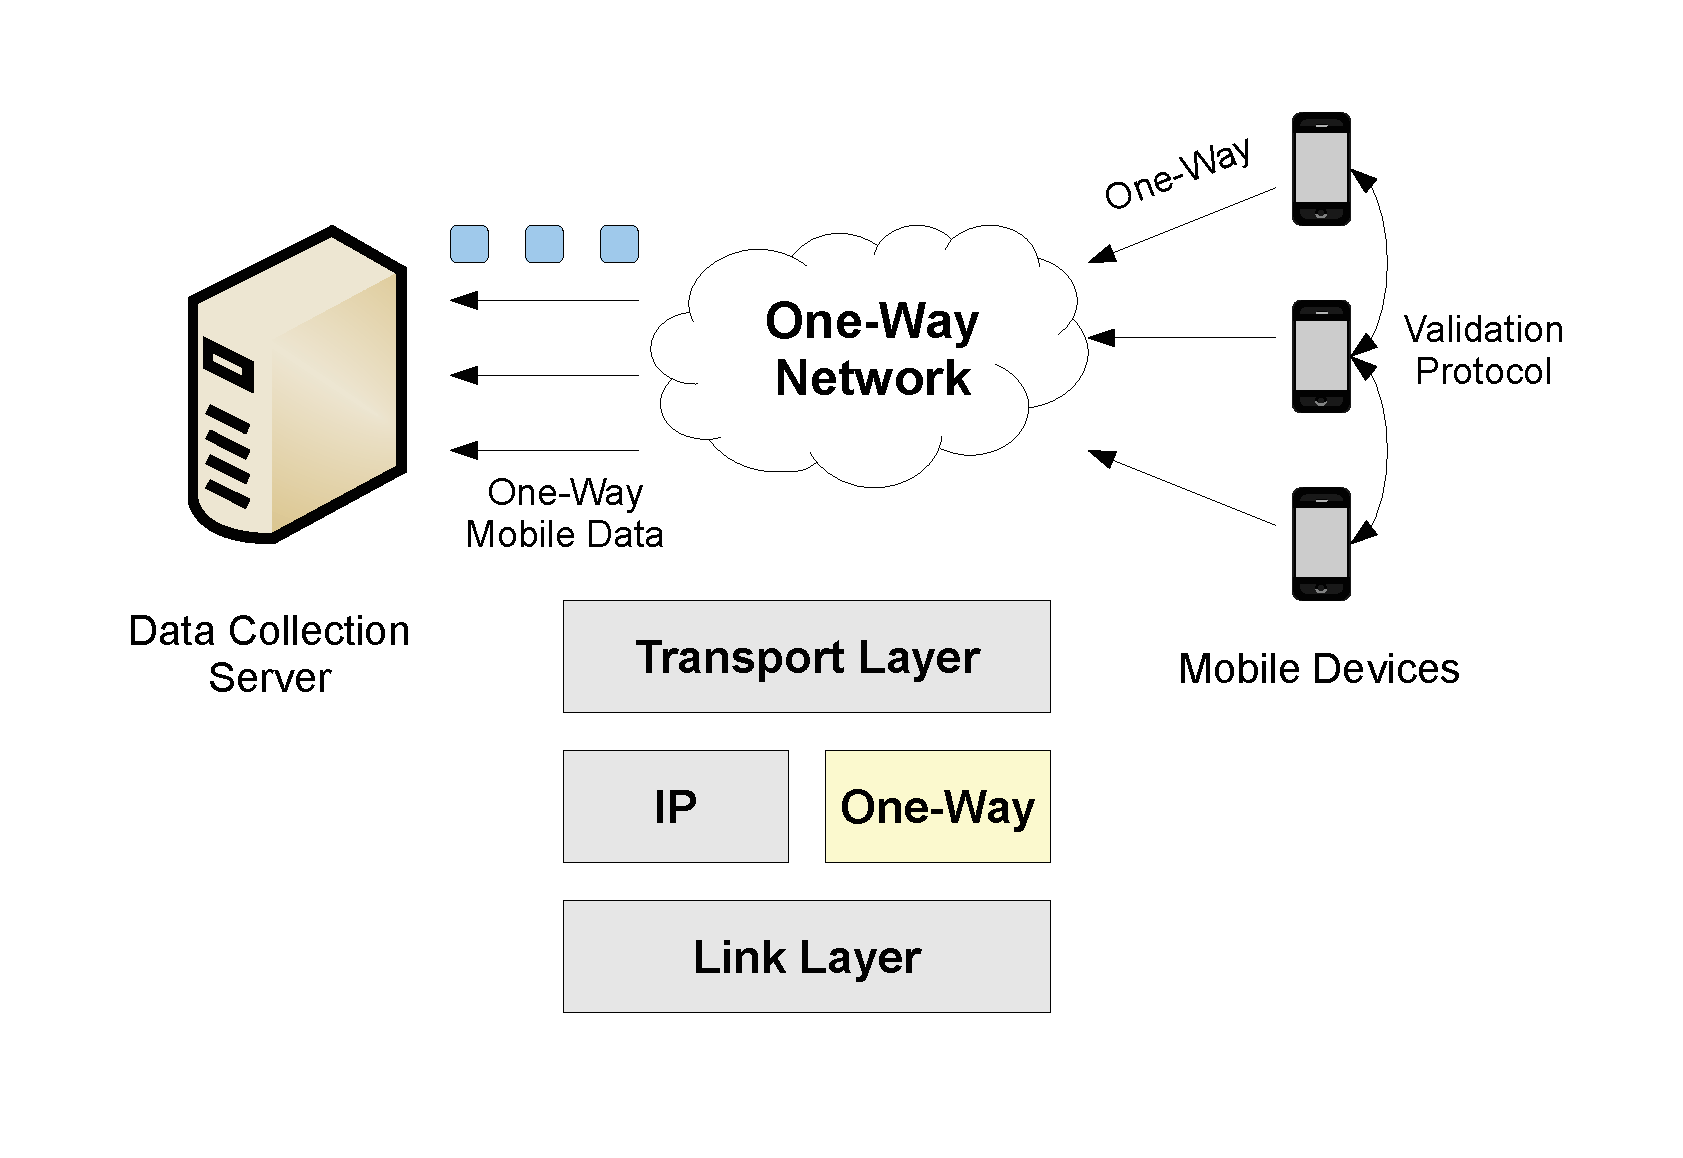
\includegraphics[width=3in]{figure1.eps}
\caption{\small \sl Anonymous Protocol.\label{fig:Stupendous}}
\end{center}
\end{figure}

\subsection{Overview}\label{proto-overview}
In this section, we describe our anonymous One-Way protocol, which completely
removes the ownership and
source information from the data transmitted to the data collection server.
Figure 1 illustrates the concept of the theoretical anonymous One-Way
protocol. One-Way is a packet routing protocol similar to the IP protocol.
Data are transmitted in packets. Each packet contains the address of the destination
host so that the packet can be correctly routed. One major difference between
One-Way protocol and other routing protocol is that, each packet does not
include the routing address of the sender (thus called One-Way). The source
address is intentionally removed so that the receiver of the data does not
know the identity of the sender. In other
words, contractually, the client does not include the source address and the
server will have no access to the source information and thus keeping the
client's identity private.

Our protocol is analogous to sending a parcel through a postal service without
sender's identity and address. An example is sending a hint to the police
pertaining a crime without revealing the sender's identity.

Unlike many other anonymous routing protocols, our protocol does not involve other
peers or mobile devices to transmit the data payload. This is particular helpful
in mobile environment in which bandwidth is limited. Some privacy aware protocols
first transmit the data payload to several mobile peers several times to mask
the identity of the sender before one of the random peers transmit the data to
the server. This puts tremendous bandwidth strain on the peers.

One drawback of a protocol without sender address is that the sender is unable
to get a feedback from the receiver whether a packet has been received (or
lost in transmission). To solve this problem, One-Way utilize a peer-to-peer
approach to verify correct transmission of a packet, much like the way
Crowds\cite{DBLP:journals/tissec/ReiterR98} uses to send data to a server.

For the validation, we want to construct a peer-to-peer network containing
$h$ nodes, where $h$ denotes the total number of hop counts for control
messages pass though. A peer node is denoted by $n_i$, meaning the
$i$th hop along the route. The peer network is a collection of nodes as
in Equation~\ref{eq:nodes}

\begin{equation}\label{eq:nodes}
\{n_0, n_1, ..., n_h\}
\end{equation}

We use $n_0$ to denote the originator of the data, and $n_h$ the last hop
that forward the data to the final receiver. For control messages travel
in the direction from sender to receiver, a node $n_i$ forwards the message
to its successor, such that $n_i \rightarrow n_{i+1}$. Similarly, for
control messages travel from the receiver back to the sender, a node 
forwards the messages to its predecessor, such that
$n_{i} \rightarrow n_{i-1}$. Table~\ref{tab:notations} summarizes the
notations used in this paper.

\begin{table}[h]
\centering
\caption{Summary of Notations} \label{tab:notations}
\begin{tabular}{c|l}
\hline
{\bf Notation} & {\bf Description}\\
\hline
$n_0$, $n_1$ ... & Peer nodes\\
$h$ & Total hop count\\
$I_s$, $I_r$ & Connection identifiers from sender and receiver, respectively\\
$A_i$, $A_r$ & Address of $i$th node and receiver, respectively\\
$D$ & Data payload\\
$s_i$ & $i$th sequence number; $s_0$ being initial sequence number\\
$c$ & Connection control message\\
$a$ & Acceptance control message\\
$p$ & Data payload message\\
$k$ & Acknowledgement control message\\
\hline
\end{tabular}
\end{table}

Opponents may argue that since the protocol resides on network layer (layer 3),
the source address could still be contained in the lower layer, e.g. the link
layer (layer 2). We argue that the source link address is different for
each hop on the route, and a route could easily contain 20 hops; therefore
the probability of tracing the link layer packet back to the original host is
really low.

\subsection{Anonymous Connection}\label{anonymous_connection}

Before transmitting data to a data collection server (receiver), the
sender makes an anonymous connection request to the server. The purpose
of the connection request is to establish a peer based route on which
acknowledgement of data transmission can be sent.

The sender initiates a connection by constructing an anonymous
connection request message, $c$. A request message contains the 
connection identifer $I_s$, routing
address (or identification), $A_r$, of the receiver,initial sequence
number $s_0$, and a hop count,
$h$. The structure of the request is defined in
Equation~\ref{eq:con_req_format}

\begin{equation}\label{eq:con_req_format}
c = \{I_s, A_r, s_0, h\}, h~\epsilon~\mathbb{N}_{\leq1}
\end{equation}

In the connection request packet, $h$ is a random natural number
denoting the number of peers the request should be forwarded to
before the request is sent to the server. The connection identifier $I_s$
is randomly generated and only last for the session and does not identify
a host.

After the sender has constructed the connection request message,
it sends the message to one of its peers running the protocol. When the
peer receives the request, it decrement the hop count $h$ by 1. If
the hop count reaches 0, then the peer sends the request to the server;
else, the peer forwards the request to another one of its peers. Note
a peer does not have to be a pure peer, but a node in the system whose
job is to facilitate communications for user nodes. Each peer in the
route keep track of the peer before and after for each request in order
to maintain the route information. If a peer declines a $c$ message,
the peer finds another peer. At the end of connection phase, the
peer-to-peer route should be constructed such that

\begin{equation}
sender(n_0) \rightarrow n_1 \rightarrow ... \rightarrow n_h \rightarrow receiver
\end{equation}

When the server receives the connection request, it sends back an acceptance
message $a$ to the node from which it receives the connection request ($n_h$).
The acceptance message contains a connection token $I_r$, as well as the
request identifier from the sender, $I_s$. The format of the acceptance
message is defined in Equation~\ref{eq:con_accept_format}

\begin{equation}\label{eq:con_accept_format}
a = \{I_r, I_s\}
\end{equation}

The node that receives the acceptance message from the receiver forwards
the message in reverse to the peer who forwarded the request message.
Each peer in the route keeps the route information based on $I_s$ and
the acceptance messages travels in revers on the same route until the
message reaches the original sender.

%[Discussion of the security of this connection approach]

%[Briefly describe routing table format and management for example, there
%is no activity for a connection for a long time. What should be done?]
\subsection{Payload Transmission}

Payload is the actual data transmitted to the server. In participatory
sensing, this is the data collected by the mobile devices from the
environment and include sensor data, photos, and videos. Payload
transmission does not involve peers since peer-forwarding in wireless
mobile environment is expensive; instead, payloads are transmitted
through the One-Way network, in which the packets only contain receiver
address and identification.

The payload transmission begins when the sender receives the acceptance
message from the server. In addition to the payload $D$, a payload
packet, denoted with $p$, also contains the address of of the receiver
$A_r$, the connection identifier $I_r$, and a sequence number $s$. The
format is defined in Equation~\ref{eq:payload_format}.

\begin{equation}\label{eq:payload_format}
p = \{A_r, I_r, s, D\}
\end{equation}

$I_r$ is the identifier issued by the server received from the connection
acceptance message. The purpose of this identifier is for the server to identify
a particular data transmission. For example, the server could be receiving
several data transmission simultaneously from different client each transmit
a file. The server assigns an identifier $I_r$ to each transmission to
differentiate the packets for the different transmissions. This field is
analogous to the port numbers in transport layers such as TCP and UDP to
multiplex packets for different connections and applications.

The sequence number $s$ in a payload packet identifies individual packets
for a transmission. The sequence numbers provide the order of the packets
and allow the receiver to identify if a packet is lost in the network, or
if packets arrived out of order.

The purpose of the connection establishment step before payload transmission
is to establish a channel in which the mobile client can verify that a packet
has been successfully received by the server. Techniques of reliable data
transfer in unreliable channel is out of scope of this paper. Reliable data
transfer mechanisms employed in TCP\cite{RFC793} and theoretical techniques
such as GO-Back-N and Select Repeat\cite{book:Kurose} can be employed with
our design. When the server wants to send a status of a packet back to
the client, it sends the status message through the peer-to-peer channel
established during connection establishment. In other words, after receiving
a payload packet $p$, the server sends an acknowledgement message, $k$, to the
node from which it received the connection request (also the node to which
it sends the connect acceptance message). Since all nodes on the anonymous route
remembers the previous node based on the connection identifiers, $I_s$ and
$I_r$, each node forwards $k$ to its previous peer until the message
reaches the originator of $p$.

%\begin{figure}[h]
%\begin{center}
%\includegraphics[width=3in]{arch.eps}
%\caption{\small \sl System Architecture.\label{fig:Stupendous}}
%\end{center}
%\end{figure}

\subsection{Node Disconnection and Failure}

When a node can no longer service a route for a connection due to
resource constraint or node shutting down, the disconnecting node (denoted
by $n_d$)
should notify its neighboring nodes of such event so that the interruption
of a connection and of delivering of control messages can be minimized.
In this section, we focus on disconnecting a single connection (as in
the case of resource constraint). If a node wishes to disconnect all
connections it supports (as in the case of node shut down), the $n_d$
performs a disconnection process discussed in this section for each
connection.

There are two scenarios for the $n_d$: the next node is an intermediate node,
and the $n_d$ is the last node in the route ($d$ = $h$).
For the first case in which the the $n_d$ is an intermediate node and the
next node is also an intermediate node, the $n_d$ should simply bridge the
gap and drop off from the route. In this case, the $n_d$ sends the node before
$n_{d-1}$
and after $n_{d+1}$
it a disconnection message containing the identity (the address)
of the two nodes. Once the connection between the two nodes has been
established, $n_d$ can remove the route information for the connection
from its routing table.

In the second case, the $n_d$ is the last node of the route and
communicates directly with the server. In this case, we do not want
just bridge the two nodes $n_{d-1}$ and $n_{d+1}$ since $n_{d-1}$
could be the originator of the data. In order to establish a new route
for the connection, $n_d$ sends a disconnection message to and telling
the server that a new control message route will be constructed for this
connection. $n_d$ also sends a route discovery message to $n_{d-1}$
and telling the node to construct a new route to the server. $n_{d-1}$
follows the same steps described in section~\ref{anonymous_connection}
to establish a new connection the the server. The connection algorithm
is detailed in Algorithm~\ref{alg:disconnect}.

\begin{algorithm}
\algsetup{linenosize=\small,linenodelimiter=. }
\caption{disconnect($n_d$)} \label{alg:disconnect}
\begin{algorithmic}[1]
\IF{$A_d$ = $A_r$}
    \STATE $m_1$ = DisconnectMessage($I_s$, $I_r$)
    \STATE $m_2$ = RediscoveryMessage($I_s$, $I_r$)
    \STATE SendToNode($A_r$, $m_1$)
    \STATE SendToNode($A_{d-1}$, $m_2$)
\ELSE
    \STATE $m_1$ = BridgeMessage($Forward$, $A_{d+1}$, $I_s$, $I_r$)
    \STATE $m_2$ = BridgeMessage($Backward$, $A_{d-1}$, $I_s$, $I_r$)
    \STATE SendToNode($A_{d-1}$, $m_1$)
    \STATE SendToNode($A_{d+1}$, $m_2$)
\ENDIF
\end{algorithmic}
\end{algorithm}

In the event of unforseen failure of a node, such as power or network
failure, the disconnected node $n_d$ is unable to notify its neighbors on
a route before disconnecting. When this happens the first thing that the
sender will notice is that it no longer receives acknowledgement message
of received packet from the server. To test for node failure in the path,
the sender $n_0$ can send a route test message into the route. When a
node $n_m$ receives the test message, it sends an acknowledgement back to
its predecessor $n_{m-1}$ on the route and forwards the test message to
its successor $n_{m+1}$ on the route. If an intermediate node on the route
$n_f$ cannot be contacted or does not acknowledge the test message, then
its predecessor $n_{f-1}$ sends a failure notice backward through the route
to notify the sender a failure has been detected. $n_{f-1}$ uses route
discovery algorithm to discovery a new route from $n_{f-1}$ to the server
and notify the new route has been successfully established. In the case
that there is no failure detected, but the sender still does not receive
acknowledgements from the server, the sender can select to terminate the
data transmission and peer connection.

\subsection{Connection Tear-Down}

After the entire file has been sent to and received by the server, the
sender can choose to tear down the connection so that the nodes can free
the resources used for the connection. To terminate a connection, the
sender injects the termination message identified by $I_s$ and $I_r$ into
the connection. Upon receiving the termination message, a node forwards
the message to its successor and free any resource associated with the
connection. Eventually the termination message reaches the server, and the
server frees the resource, and stores the received file.


%\section{Related Work}\label{sec-relwork}
%\input{related}

%\section{System Architecture}\label{sec-design}
%


%\section{Experimental Validation}\label{sec-experiment}
%\input{experiments}

%\section{Conclusions}\label{sec-conc}
%\input{conc}

%\section{Acknowledgements}\label{sec-ack}
%\input{ack}


\setstretch{1}{
\bibliographystyle{plain}
\bibliography{Jeff_citations}
\end{document}
